\thispagestyle{empty}
\refstepcounter{dummy}
\addcontentsline{toc}{chapter}{\tocEntry{Paper I}}
%*******************************************************
\topskip0pt
\vspace*{\fill}
\begin{flushright}
\Huge{\textbf{Paper I}}
\end{flushright}

\Large{
\textsc{Four-Component Relativistic Calculations in Solution with the
Polarizable Continuum Model of Solvation: Theory,
Implementation, and Application to the
Group 16 Dihydrides
\ce{H2X} (\ce{X} = \ce{O}, \ce{S}, \ce{Se}, \ce{Te},
    \ce{Po})}
\\
\textbf{R. Di Remigio}, R. Bast, L. Frediani, and T. Saue
\\
\textit{J. Phys. Chem. A}, \textrm{2015}, \textbf{119}, 5061--5077
}
\vspace*{\fill}

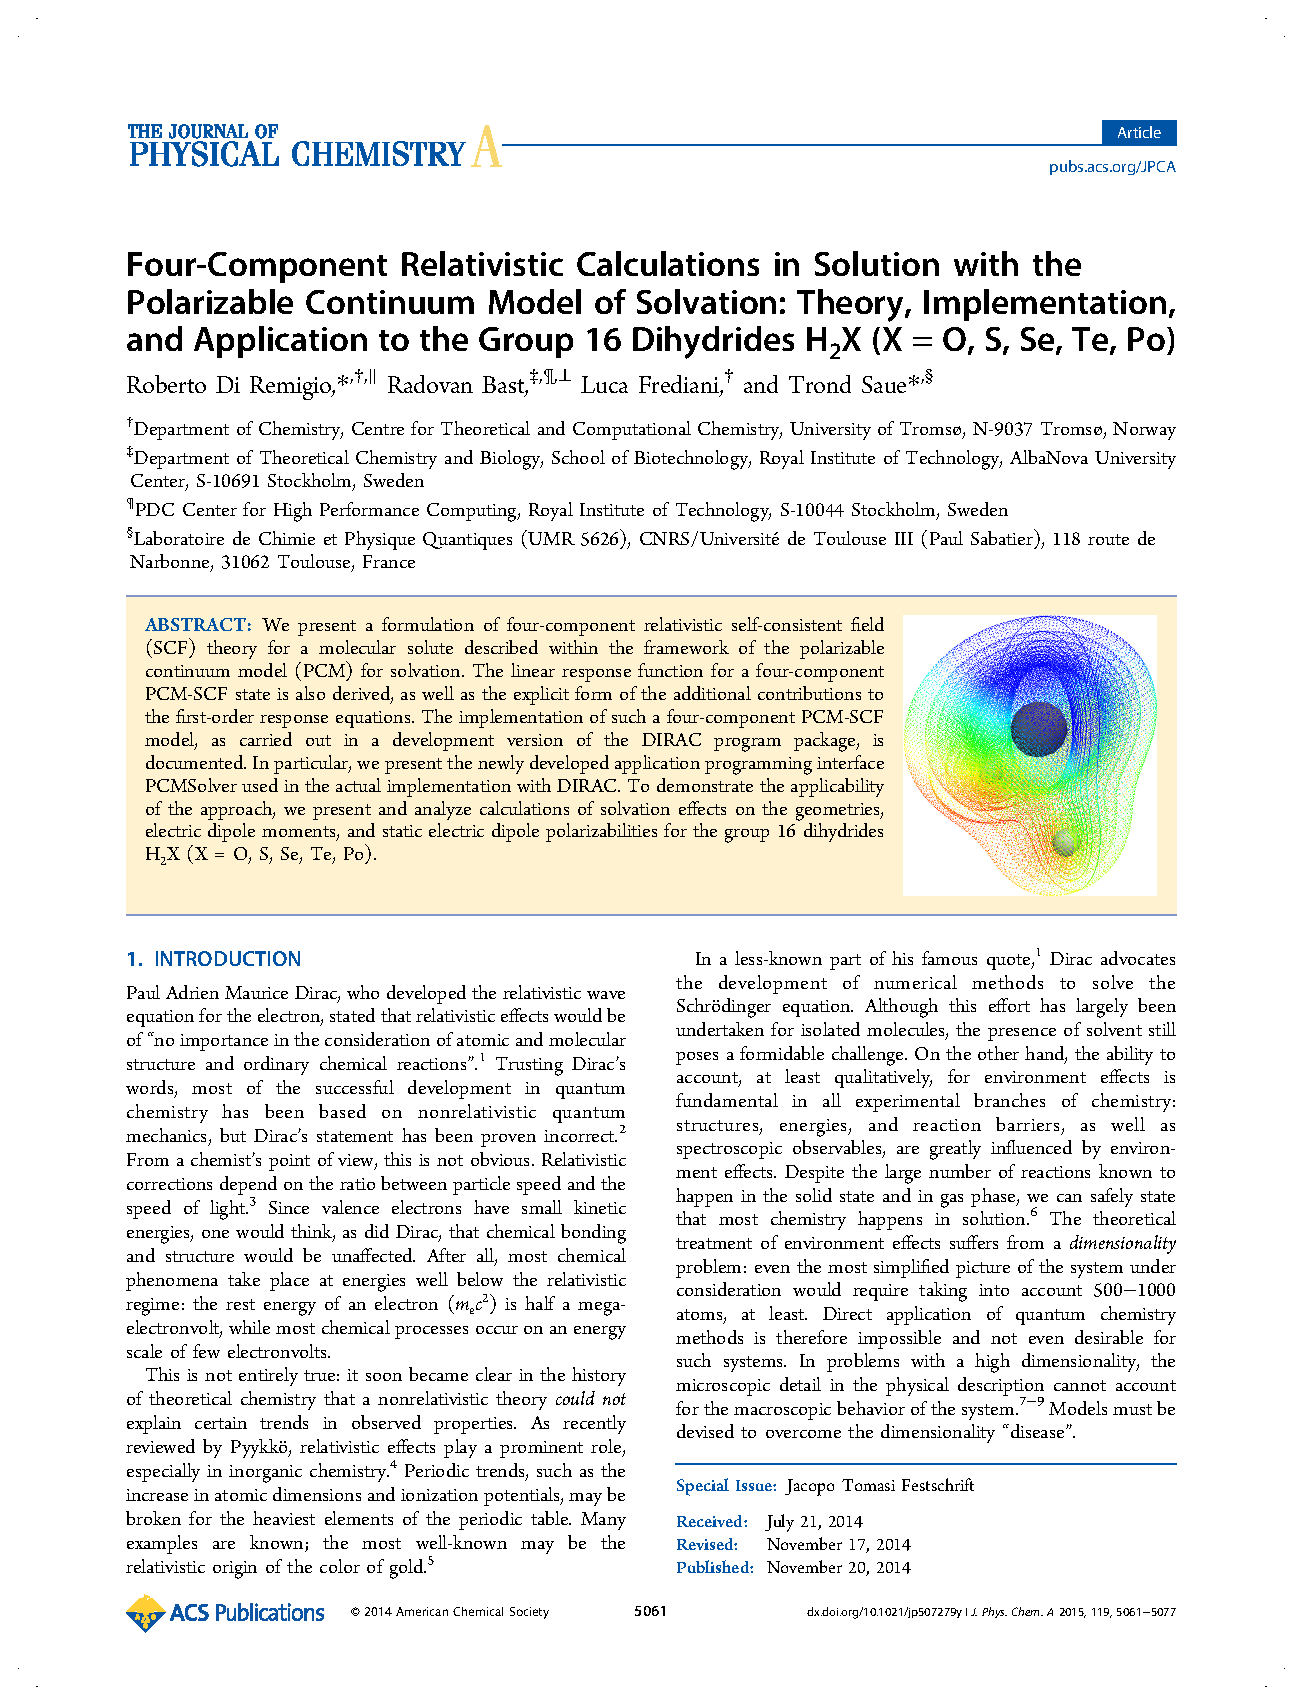
\includepdf[pages=-]{papers/relapcm.pdf}

\thispagestyle{empty}
\refstepcounter{dummy}
\addcontentsline{toc}{chapter}{\tocEntry{Paper II}}
%*******************************************************
\topskip0pt
\vspace*{\fill}
\begin{flushright}
\Huge{\textbf{Paper I}}
\end{flushright}

\Large{
\textsc{
Wavelet Formulation of the Polarizable Continuum Model. II. Use of Piecewise
Bilinear Boundary Elements
}
\\
M. Bugeanu, \textbf{R. Di Remigio}, K. Mozgawa, S. S. Reine, H.
Harbrecht,  and L. Frediani
\\
\textit{Phys. Chem. Chem. Phys.}, \textrm{2015}, \textbf{17},
31566--31581
}
\vspace*{\fill}

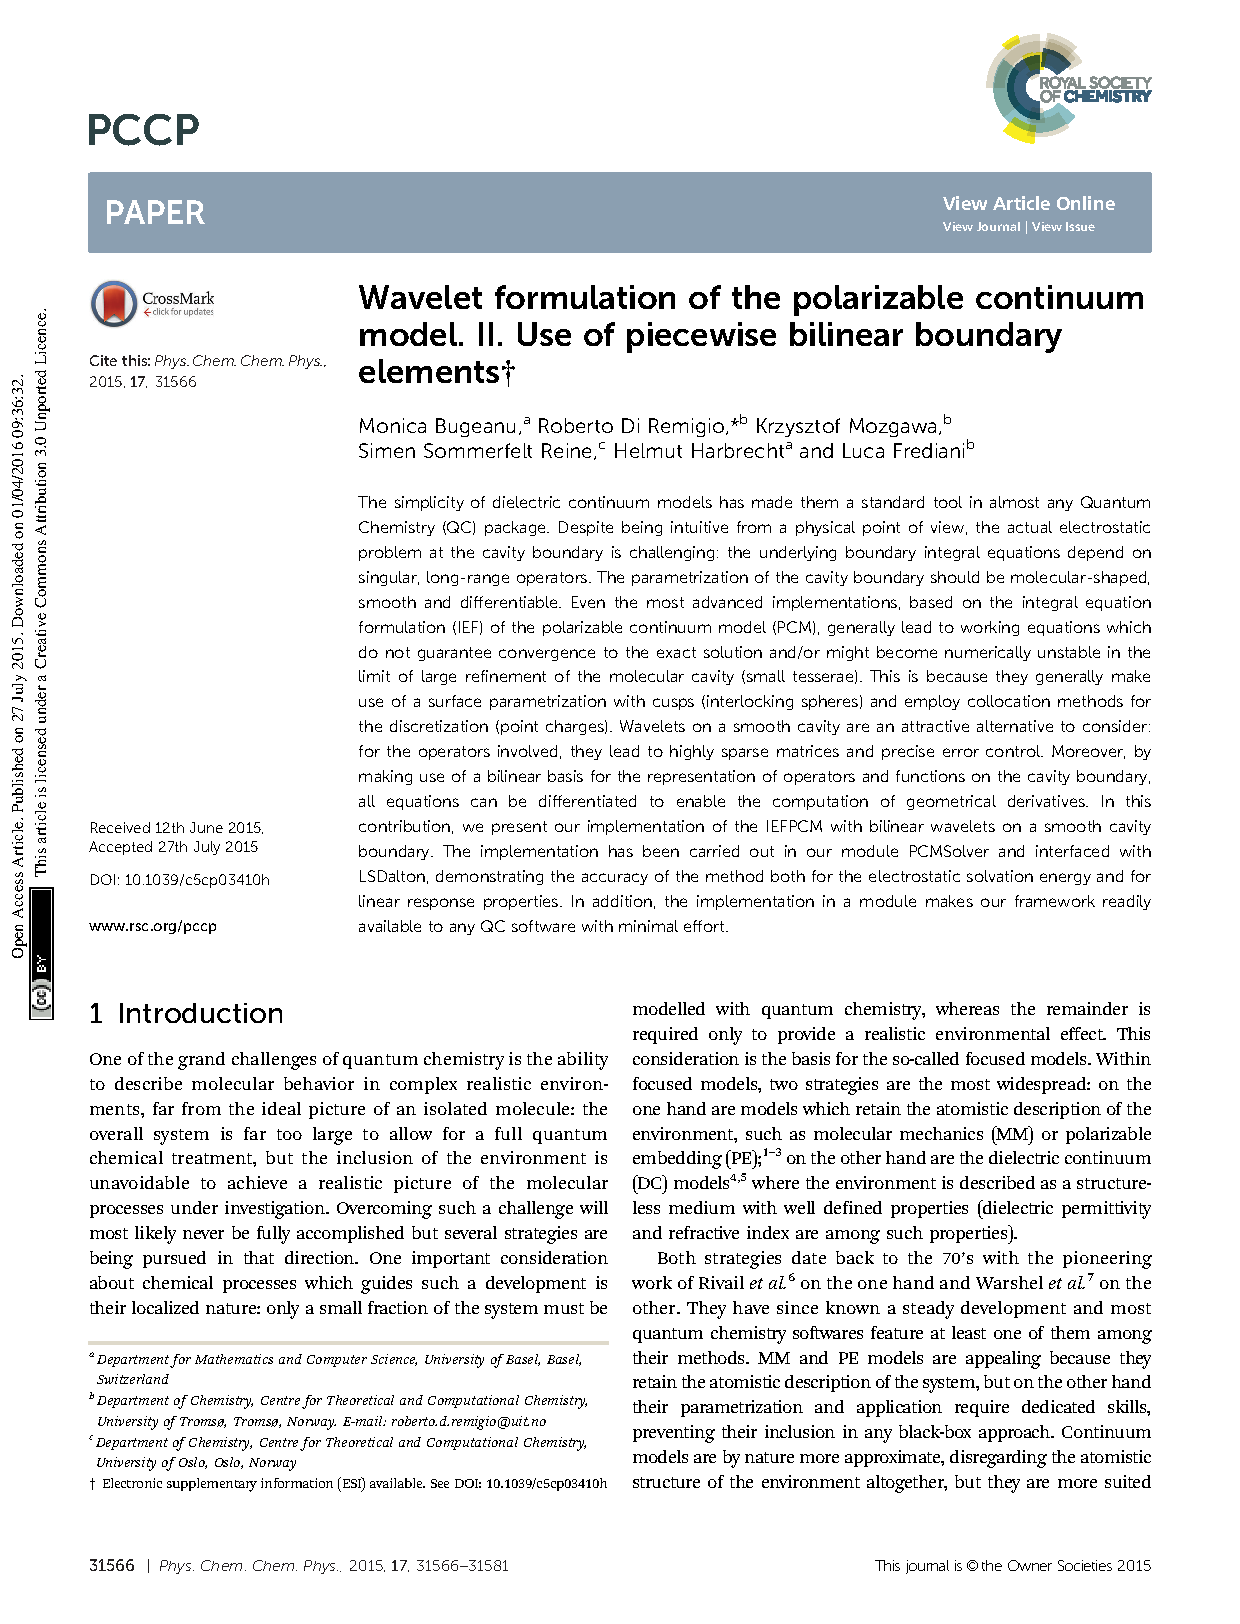
\includepdf[pages=-]{papers/wemlin.pdf}

\thispagestyle{empty}
\refstepcounter{dummy}
\addcontentsline{toc}{chapter}{\tocEntry{Paper III}}
%*******************************************************
\topskip0pt
\vspace*{\fill}
\begin{flushright}
\Huge{\textbf{Paper I}}
\end{flushright}

\Large{
\textsc{
    A Polarizable Continuum Model for Molecules at Spherical
    Diffuse Interfaces
}
\\
    \textbf{R. Di Remigio}, K. Mozgawa, H. Cao, V. Weijo, and L.
    Frediani
\\
    \textit{J. Chem. Phys.}, \textrm{2016}, \textbf{144}, 124103
}
\vspace*{\fill}

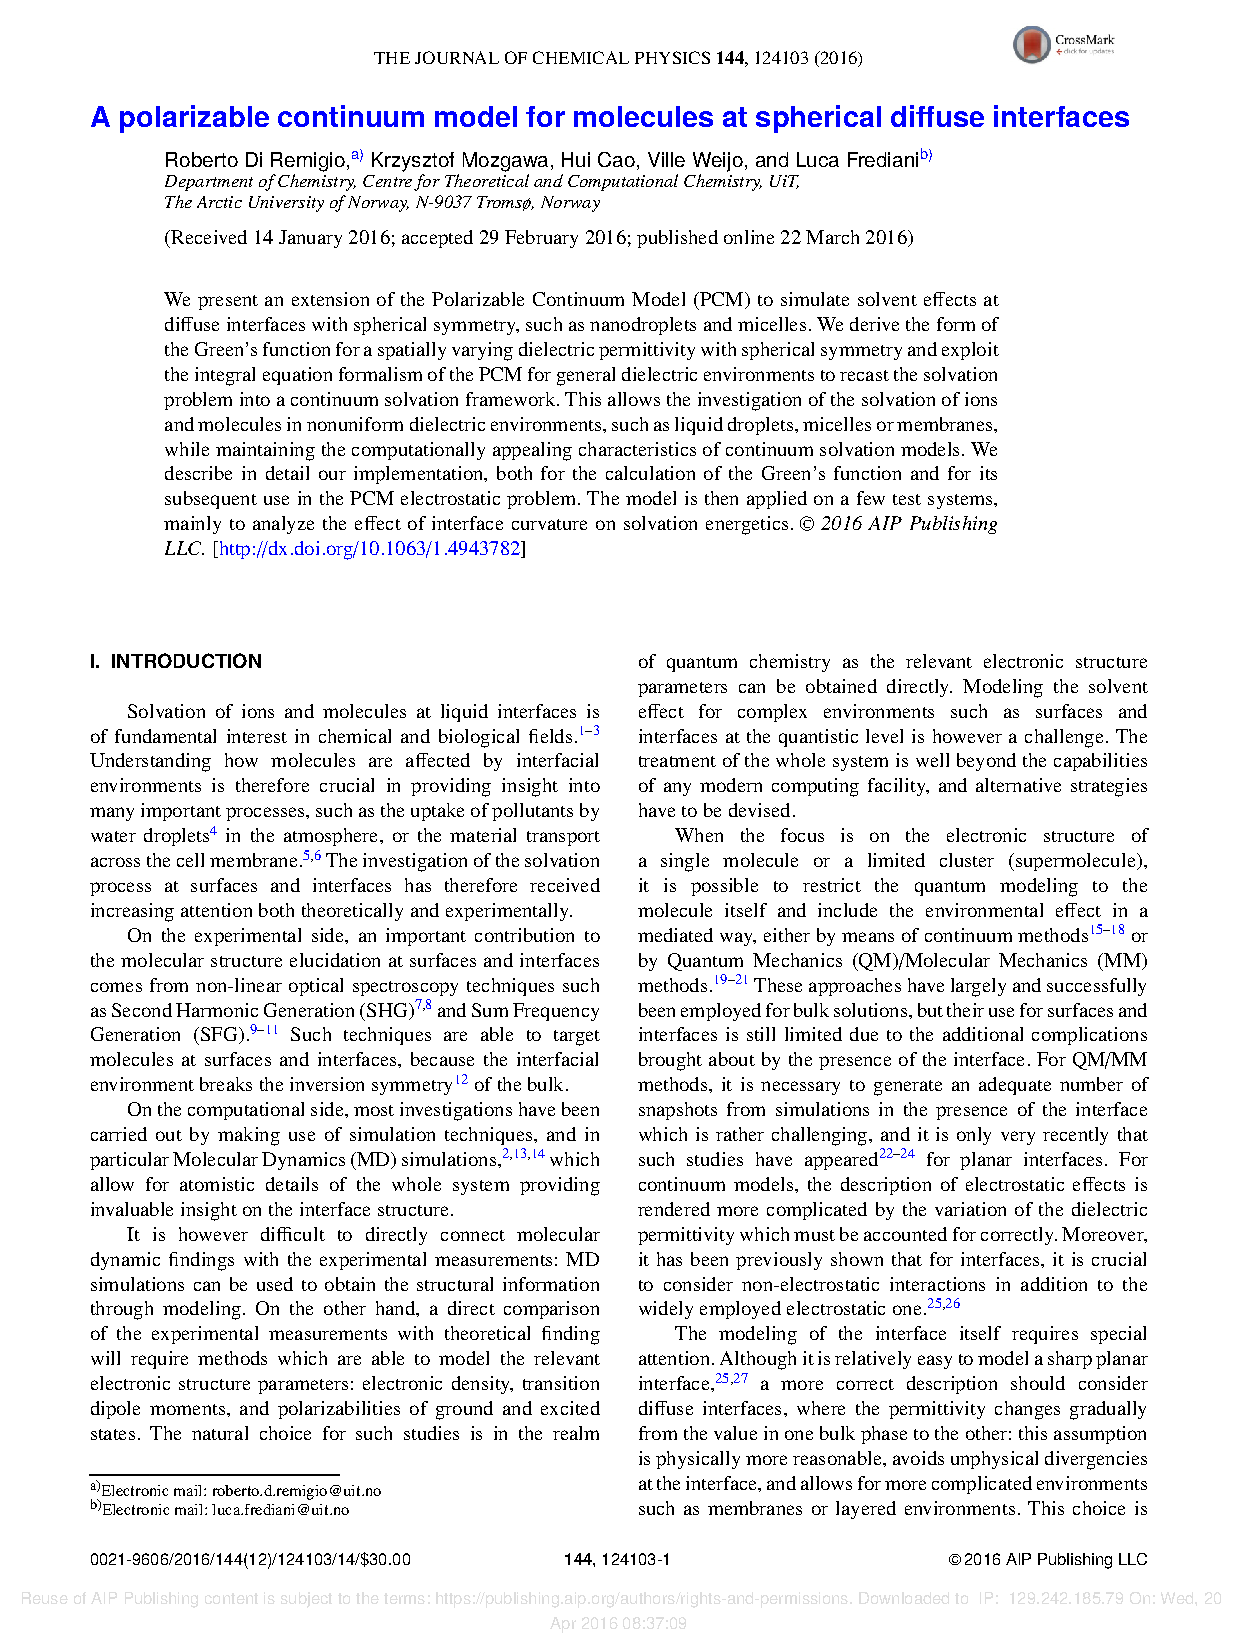
\includepdf[pages=-]{papers/spherical.pdf}
